% LaTeX report template 
%

% This is a comment: in LaTeX everything that in a line comes
% after a "%" symbol is treated as comment

\documentclass[11pt, a4paper]{article}
\usepackage{graphicx}
\usepackage{amsmath}
\usepackage{listings}
\usepackage{geometry}
\usepackage[utf8]{inputenc}

\geometry{
 a4paper,
 total={170mm,257mm},
 left=20mm,
 top=20mm,
 }

\title{Assignment 5: The Resistor Problem} % Title

\author{JINEETH N [EE20B051]} % Author name

\date{March 9,2022} % Date for the report
\begin{document}	
\lstset{language=Python}
	
\maketitle % Insert the title, author and date		
  \section*{Abstract}
  \begin{itemize}
  \item
  	To solve for potential and currents in a system.
  \item
  	To solve 2-D Laplace equations in an iterative manner.
  \item
	To plot graphs to understand the 2-D Laplace equation.	
\end{itemize}  	
  
  \section{Introduction}
  A wire is soldered to the middle of a copper plate and its voltage is held at 1 Volt. One side of the plate is
    
       Ohm's law   
    \begin{equation}
    \vec{J} = \sigma\vec{E}
       \end{equation}
    
      Charge Continuity equation.
    \begin{equation}
    \nabla.\vec{J} = -\frac{\partial \rho}{\partial t}
       \end{equation}
    
      From the above equations,

    \begin{equation}
    \nabla^{2}\phi = \frac{1}{\sigma}\frac{\partial \rho}{\partial t}
       \end{equation}

      For DC currents, the right side is zero, and we obtain

    
    \begin{equation}
    \nabla^{2}\phi = 0
       \end{equation}


  \section{Tasks}
 
 \subsection{Parameters}
 They are assigned default values, which will be corrected via commandline arguments
    \begin{verbatim}
    Niter = 1500
    Ny = 25
    Nx = 25
    radius = 8

# The above parameters can also be given through the commmand line.
if len(sys.argv) > 1:
    Nx = sys.argv[1]
    Ny = sys.argv[2]
    Niter = sys.argv[3]

n = arange(Niter)

    \end{verbatim}
    
\subsection{Variable initialization}
Create a zero 2-D array of size Nx x Ny and assign 1 to cordinates within radius 1 from center
\begin{verbatim}
    phi = np.zeros((Ny, Nx))

    rng = 0.5
    y = np.linspace(-rng, rng, Ny)
    x = np.linspace(-rng, rng, Nx)
    X, Y = meshgrid(x, -y)

\end{verbatim}

\subsection{Allocating potential and plotting it}
\begin{verbatim}
    # Assign potential = 1
    ii = where(((X * X) + (Y * Y)) <= (0.35 * 0.35))
    phi[ii] = 1.0
    
    plt.plot(x[ii[0]], y[ii[1]], "or", label="V = 1")
\end{verbatim}

\begin{figure}[!ht]
  \centering
  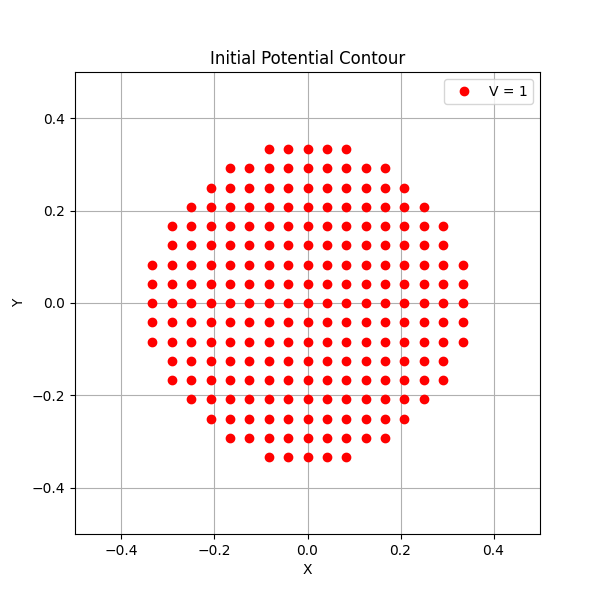
\includegraphics[scale=0.7]{Figure_1.png}
  \caption{semilogy scale}
  \label{fig:sample}
 \end{figure}
 
 \subsection{Updating Potential}
 After converting the equation(4) to discrete domain, we can update matrix through iterations
  \begin{equation}
            \phi_{i,j} = \frac{\phi_{i+1,j} + \phi_{i-1,j} + \phi_{i,j+1} + \phi_{i,j-1}}{4} 
    \end{equation}
The bottom boundary is grounded. The other 3 boundaries have a normal potential of zero
\begin{verbatim}
    errors = np.zeros((Niter, 1))
for k in range(Niter):
    oldphi = phi.copy()
    phi[1:-1, 1:-1] = (1/4) * (
        phi[1:-1, 0:-2] + phi[1:-1, 2:] + phi[0:-2, 1:-1] + phi[2:, 1:-1]
    )

    # These lines will set the proper boundary conditions.
    phi[1:-1, 0] = phi[1:-1, 1]
    phi[1:-1, -1] = phi[1:-1, -2]
    phi[0, 1:-1] = phi[1, 1:-1]
    phi[ii] = 1.0
    errors[k] = (abs(phi - oldphi)).max()
\end{verbatim}

\begin{itemize}
    \item 
we can observe that error decreases linearly for higher no of iterations,so from this we conclude that for large iterations error decreases exponentially with No of iterations i.e it follows AeBx as it is a semilog plot

And if we observe loglog plot the error is almost linearly decreasing for smaller no of iterations
so it follows ax form since it is loglog plot and follows some other pattern at larger iterations.
\end{itemize}

\subsection{Plotting the errors}
We will plot the errors on semi-log and log-log plots. We can observe the error decreases very slow
\begin{verbatim}
    
    loglog(n, errors)
    
    
    semilogy(n[500:], errors[500:])
    
\end{verbatim}

\begin{figure}
\centering
\begin{minipage}{.5\textwidth}
  \centering
  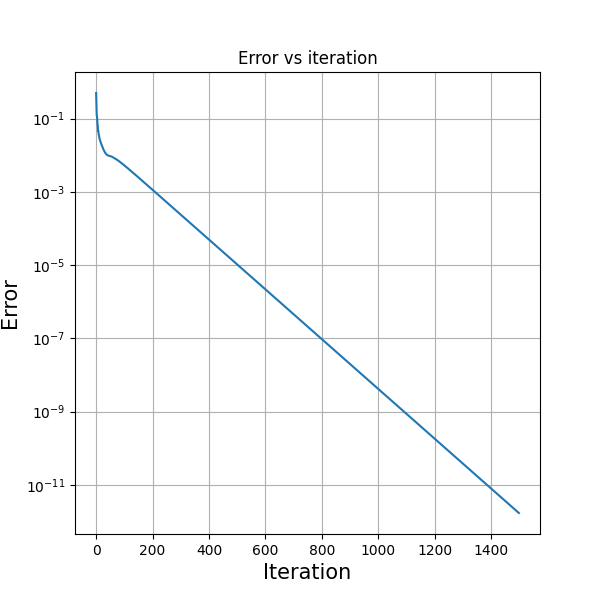
\includegraphics[scale=0.6]{Figure_2.png}
  \caption{Error (semilog)}
  \label{fig:sample}
\end{minipage}%
\begin{minipage}{.5\textwidth}
  \centering
  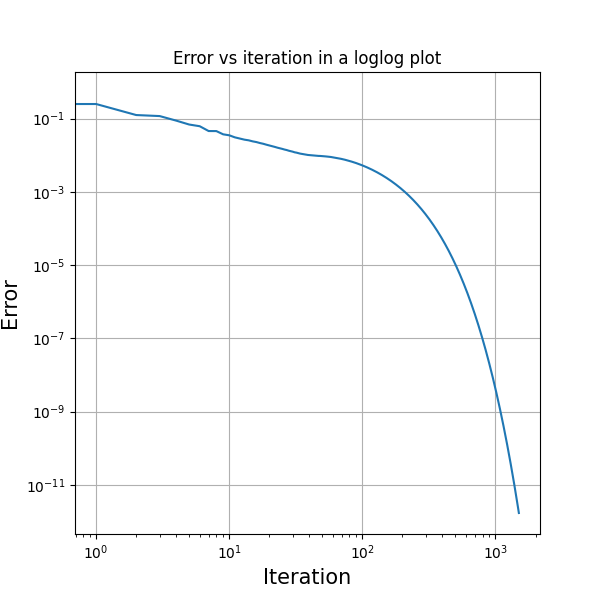
\includegraphics[scale=0.6]{Figure_3.png}
  \caption{Error (loglog)}
  \label{fig:sample}
\end{minipage}
\end{figure}

\subsubsection{Fitting exponential curve}
We observed that the error is decaying exponentially for higher iterations. We will fit two curves.

\begin{figure}[!ht]
  \centering
  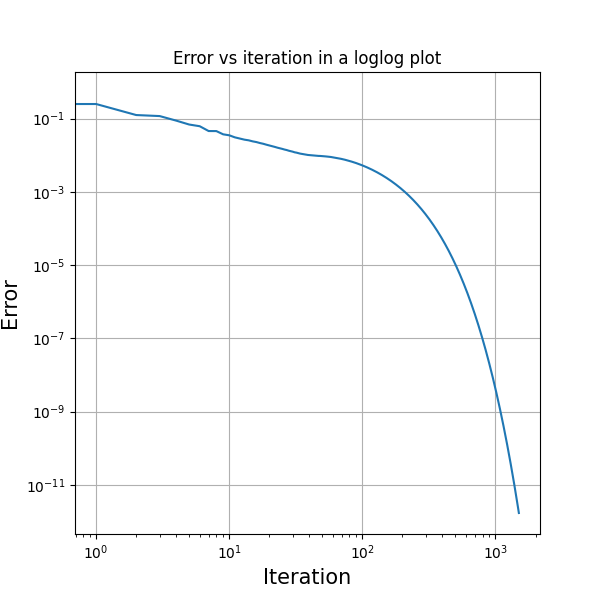
\includegraphics[scale=0.8]{Figure_3.png}
  \caption{Potting exponential curves}
  \label{fig:sample}
  \end{figure}
 \subsection{Plotting Potential}
 \begin{verbatim}
    # Contour plot of potential
    plt.title("Contour plot of V", fontsize=16)
    plt.contourf(Y, X[::-1], phi)
    plt.plot(x[ii[0]], y[ii[1]], "or", label="V = 1")
    
\begin{verbatim}
    # The exponent part of the error values can be got using the below piece of code.
y1 = log(errors)
yfit = lstsq(c_[np.ones(Niter - 0), arange(Niter - 0)], y1, rcond=None)[0]
#fitting a straight line in log scale and calculating actual values in normal scale
a, b = exp(yfit[0]), yfit[1]
y2 = log(errors[500:])
yfit = lstsq(c_[np.ones(Niter - 500), arange(500, Niter)], y2, rcond=None)[0]
a_500, b_500 = exp(yfit[0]), yfit[1]

\end{verbatim}


\begin{itemize}
    \item Considering all iteration
    \item Considering after 500th iteration
\end{itemize}



\begin{figure}
  \centering
  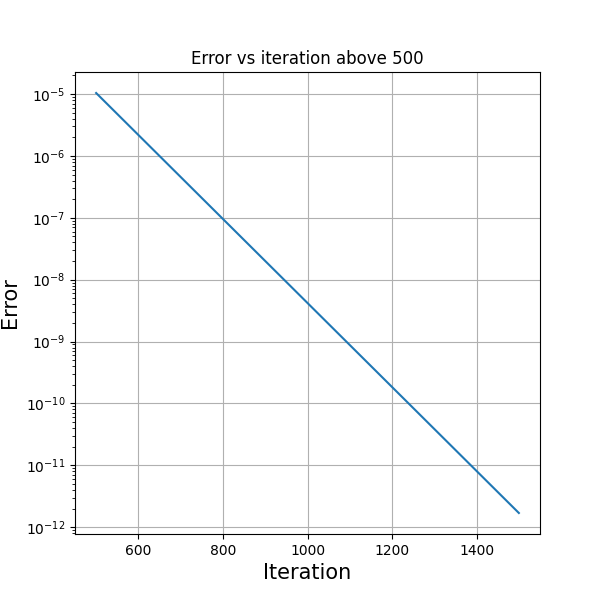
\includegraphics[scale=0.8]{Figure_4.png}
  \caption{Potting exponential curves}
  \label{fig:sample}
  \end{figure}
 
 
 \subsection{Plotting Potential}
 
\begin{verbatim}
    
figure(7, figsize=(6, 6))
contourf(X, Y, phi)
plot(xp, yp, "ro", label="V = 1")
xlabel(r"X")
ylabel(r"Y")
title("Contour plot of potential")
grid()
legend()


fig1 = figure(8, figsize=(6, 6))
ax = p3.Axes3D(fig1)
xlabel(r"X")
ylabel(r"Y")
title("The 3-D surface plot of the potential")
surf = ax.plot_surface(X, Y, phi, rstride=1, cstride=1, cmap=cm.jet)
\end{verbatim}
 
 \begin{figure}
  \centering
  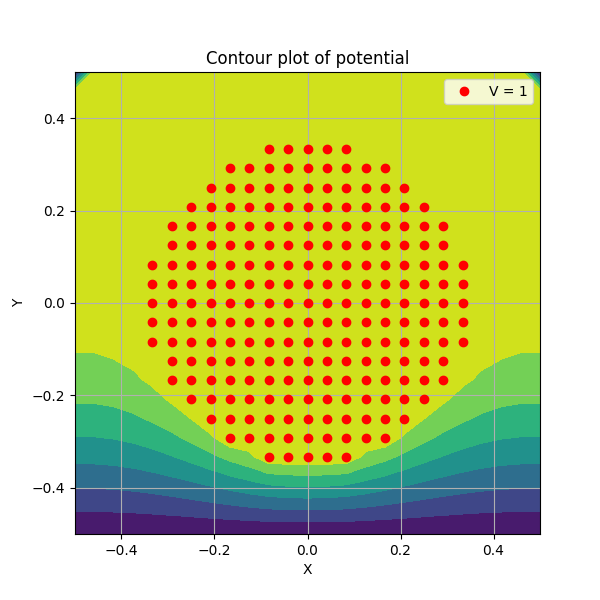
\includegraphics[scale=0.8]{Figure_7.png}
  \caption{Contour plot of potential}
  \label{fig:sample}
   \end{figure}
   
\begin{figure}[!ht]
  \centering
  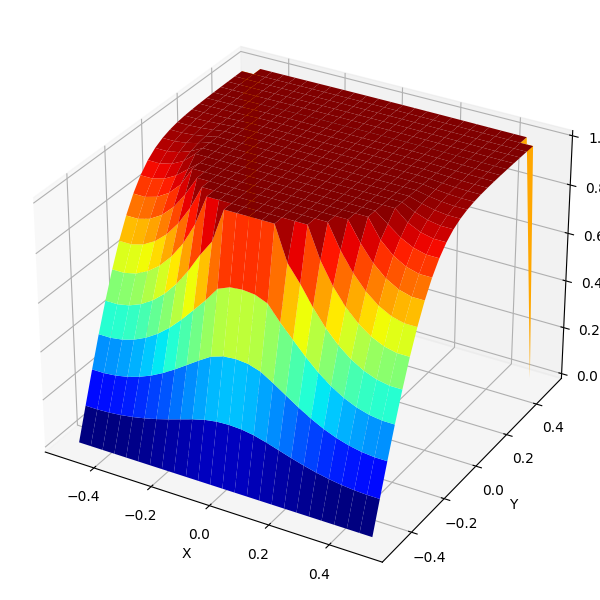
\includegraphics[scale=0.8]{Figure_8.png}
  \caption{3D Potential plot}
  \label{fig:sample}
   \end{figure}
   
 \newpage
 \subsection{Vector plot of currents}
 We use the below equations to calculate current,
 \begin{equation}
        J_{x,ij} = \frac{1}{2}(\phi_{i,j-1} - \phi_{i,j+1}) 
    \end{equation}

\begin{equation}
        J_{y,ij} = \frac{1}{2}(\phi_{i-1,j} - \phi_{i+1,j}) 
    \end{equation}

\begin{verbatim}
Jx = np.zeros((Ny, Nx))
Jy = np.zeros((Ny, Nx))
Jx = 0.5 * (phi[1:-1, 0:-2] - phi[1:-1, 2:])
Jy = 0.5 * (phi[2:, 1:-1] - phi[0:-2, 1:-1])


figure(9, figsize=(6, 6))
quiver(X[1:-1, 1:-1], Y[1:-1, 1:-1], Jx, Jy)  
plot(xp, yp, "ro")
xlabel(r"X")
ylabel(r"Y")
title("The vector plot of the current flow")
\end{verbatim}


\begin{figure}
  \centering
  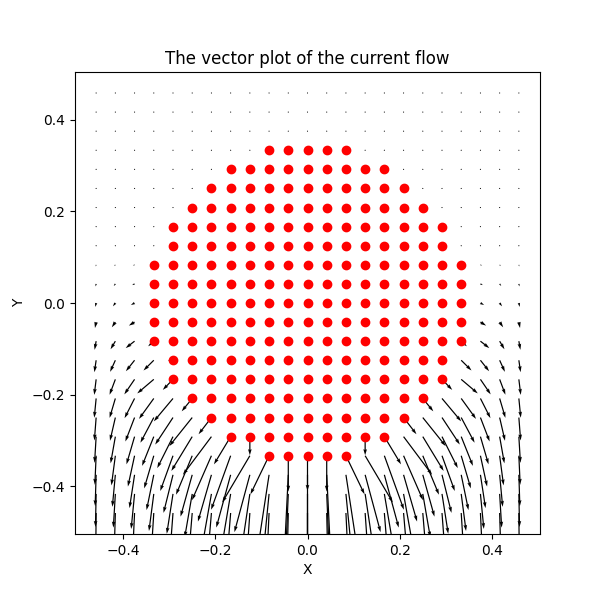
\includegraphics[scale=0.8]{Figure_9.png}
  \caption{Current vectors}
  \label{fig:sample}
   \end{figure}
  
 \newpage
\section{Conclusion}
\begin{itemize}
  \item
    Most of the current is restricted to bottom part of the wire and it is normal to the surface of both wire and metal
  \item
    We can vectorize multiple "for" loops to a single line in python
  \item
    Also we observed that the decrease in error is very slow after 500 iterations which makes this method inefficient
  \end{itemize}



  \end{document}
